\section{Registration measures follow-through; the use-proof gate measures survival}\label{sec:life}

A US trademark passes through a sequence of dated, high-stakes steps, and
each step leaves a record. An application is filed with a goods/services
description; an examiner reviews it, often issuing office actions the
applicant must answer; if allowed and (for intent-to-use filings) a
statement of use is filed, the mark registers. Registration starts a
maintenance clock: in years five to six the owner must file a Section~8
declaration proving continued use in commerce, with a six-month grace
period; around year ten a combined Section~8 declaration and Section~9
renewal is due, and every ten years thereafter. A mark that misses a
use-proof gate is cancelled. Madrid Protocol registrations
(\S66(a) basis) file Section~71 declarations on the same schedule and
are flagged separately throughout. \citet{Graham2013} describe the
administrative data; the event-dated corpus built here adds the full
prosecution history of each case, so a cancellation is assigned to a
specific gate by its date rather than inferred from a status snapshot.

\begin{table}[h]\centering\small
\caption{The trademark funnel in this corpus. Registration counts are
unique serials; gate outcomes are event-dated (a Section~8 cancellation
at registration age 4.0--8.5 years). Source: the re-parsed USPTO
application backfile, scored as in Section~\ref{sec:construct}.}
\label{tab:funnel}
\begin{tabular}{lrr}
\toprule
Stage & $n$ & Share \\
\midrule
Debut filings scored, 1995--2018 (owners' first filings) & 3{,}589{,}068 & \\
\quad reached registration & 2{,}066{,}600 & 57.6\% \\
\midrule
All unregistered class-records filed 1995--2018 & 3{,}798{,}318 & \\
\quad never filed statement of use & & 42.6\% \\
\quad stopped responding in prosecution & & 45.3\% \\
\quad removed adversarially & & 4.3\% \\
\midrule
Registrations 2002--2018, scored, unique serials & 3{,}104{,}534 & \\
\quad failed the first use-proof gate (event-dated) & & 52.3\% \\
\midrule
Passed first gate, cohorts 2002--2013, terminal status known & 1{,}129{,}724 & \\
\quad failed at the year-ten renewal & & 39.1\% \\
\bottomrule
\end{tabular}
\end{table}

The paper relates two properties of a filing's description --- how unusual
its language is for its industry, its \emph{atypicality}, and whether that
language is ahead of or behind where the industry's language was moving, its
\emph{lead} --- to what happened to the filing afterwards. Section~\ref{sec:construct}
builds the two properties. The outcomes are three steps in the sequence above,
each read from the dated record and each bounded as follows.

\emph{Registration.} Whether an application reaches registration at all,
among filings made 1995--2018. Of the applications that do not register,
roughly nine in ten die by the applicant's own inaction --- never filing the statement of use, or going
silent during prosecution --- and only 4.3\% are removed adversarially
(Table~\ref{tab:funnel}), so registration is read as a launch indicator rather
than an examiner's verdict.

\emph{Survival of the first use-proof gate.} Whether a registration was
cancelled for non-use at registration age 4.0 to 8.5 years, among
registrations issued 2002--2018. This is where the market's verdict reaches
the record: half of registered marks do not survive it, and failing it means
the product the mark named is no longer in commerce. Every gate estimate is
conditional on the mark having been granted, because registration is itself
selected on language; what the unconditional composite looks like is shown
once, in Appendix~\ref{app:uncond}, and not otherwise used.

\emph{Reaching SEC reporting.} Whether the owner of a first-time filing ever
appears in SEC financial-statement records, a firm-level outcome used in
Section~\ref{sec:bluesea} to ask whether either property of the text marks
firms bound for public markets.

Outcomes are rates, so every estimate is a shift in a probability and is
stated in percentage points against the base rate it shifts: $+1.4$pp on a
52.3\% base means 53.7\% against 52.3\%, not 52.3\% multiplied by $1.014$.
The basic comparison is the outcome rate of the fifth of filings with the
highest lead minus that of the fifth with the lowest, with the fifths cut
inside a single industry and year so that no difference between industries or
between years enters; the regression tables add drafting and filer controls
and cluster errors on the owner. Where a continuous version is given, it is
the change in the outcome for a one-standard-deviation change in lead, in
percentage points.

Counting differs by table. A filing may claim several Nice classes at once, so
a \emph{class-record} counts it once per class while a \emph{registration}
counts it once by serial number; a \emph{debut filing} is an owner's first, one
per owner. The funnel above counts debut filings, the gate regressions unique
registrations, the per-class figures class-records.

Three windows bound the samples, each set by an institutional fact. Scoring
runs 1995--2019, because a full
five-year past reference does not exist before 1990 and a full forward
reference does not exist after 2020; the analysis cut of 1995 is about two
years more conservative than the measured burn-in requires
(Appendix~\ref{app:comp}). The gate cohorts end in 2018 because the
cancellation record runs to April 2026 and the failure window closes at
registration age 8.5 years, so 2018 is the last cohort whose window has
essentially elapsed --- the top of that range is fractionally censored, and
a separate 2019 replication is reported below. They begin in 2002 because
that is the conventional cut for this corpus, and that lower
bound turns out to matter: carried back to the first scoreable cohorts the
penalty is two to three times larger than it has ever been since, and
Section~\ref{sec:eras} reports what the restricted window concealed.

Outcomes are read from the event-dated prosecution history, which attributes
each cancellation to a specific gate and observes counsel and basis directly,
and cross-checked against the USPTO status-code dictionary.\footnote{700
registered; 701--705 Section~8 accepted; 710 cancelled for Section~8 failure;
800 renewed; 900 expired.}

% The construct section lives in its own file so it can be revised
% independently; see paper/section_construct.tex.
% ---------------------------------------------------------------------------
% Standalone construct section, meant to be % ---------------------------------------------------------------------------
% Standalone construct section, meant to be % ---------------------------------------------------------------------------
% Standalone construct section, meant to be \input{section_construct} from
% ssrn_diffusion_paper.tex so it can be revised independently of the rest.
%
% Depends on the host preamble for: \dkl{} (defined as $\Delta$KL), natbib,
% booktabs, amsmath. Citation keys used here all exist in the host
% bibliography: Murdock2017, Barron2018, vonGraevenitz2022.
%
% Naming decided 2026-08-06 after consultation. The signed axis is LEAD, and
% filings are LEADING or LAGGING; "currency" was rejected because readers
% import monetary logic into what is a claim about lexical surprise, and
% "resonance" because it names a mechanism this design cannot observe.
% ---------------------------------------------------------------------------

\section{The construct: how surprising a description is, and when}\label{sec:construct}

\subsection{Two questions asked of every filing}

The measure asks one thing twice. Take a filing's goods/services description,
and group every filing by its Nice class --- one of the 45 international goods
and services categories --- and by its year. Then ask:

\begin{enumerate}[noitemsep]
  \item How surprising would this wording have been to a reader who knew only
        what that industry had filed over the previous five years?
  \item How surprising does the same wording look to a reader who also knows
        what the industry filed over the following five years?
\end{enumerate}

\noindent The two answers are rarely the same, and the gap between them is
informative. Wording that was surprising when filed and unremarkable five
years later was surprising because it came first: the industry moved toward
it. Wording that read as ordinary when filed and unusual afterwards was behind
its industry rather than ahead of it, and was left behind as the field moved
on. Filings of the first kind are \emph{leading}; of the second,
\emph{lagging}.

Both quantities are computable for every filing in the corpus, including the
millions from firms that never patent, and neither requires knowing anything
about the firm.

\subsection{Antecedents, and what does not carry over}

The apparatus is that of \citet{Murdock2017}, developed on Darwin's reading
notebooks, and \citet{Barron2018}, who extended it to French Revolution
parliamentary debates. They score each document against the distribution of
documents before it and again against the distribution after it, and call the
two quantities \emph{novelty} and \emph{transience} and their signed difference
\emph{resonance}.

The arithmetic transfers exactly. The interpretation does not, in two ways that
shape everything downstream.

First, there is no single authoring agent. In a reading notebook the author of
the document is the person whose novelty is being measured, and the reference
stream is that author's own intellectual environment; a high value therefore
says something about a mind. Here each filing is scored against the stream of
\emph{other} firms' filings, and the author is typically counsel drafting for
scope of protection. The same number can only say that a description sits far
from what its industry was writing.

Second, \emph{resonance} names a mechanism this design cannot observe. A filing
can sit where its class was heading because it was imitated, because it and the
class responded to the same external development, or by coincidence, and
nothing here separates those. The vocabulary used below is therefore positional
rather than causal: a leading filing was ahead of its industry's language,
which implies the existence of a trajectory without asserting that the filing
caused it.

The nearest measurement precedent on this corpus is \citet{vonGraevenitz2022},
who flag goods/services tokens that are both new and fast-spreading and use
their geography to study diffusion. Their unit is the token and their novelty
flag is binary, assigned once a token's path is known; the measure here is
continuous and attaches to the filing, so every application carries a position
and that position can be crossed with the mark's own prosecution outcomes.

\subsection{Definitions}

Let $P_t$ be the topic distribution of a filing made in year $t$, and let
$Q_{\mathrm{past}}$ and $Q_{\mathrm{future}}$ aggregate same-class filings over
the $W = 5$ years before and after it. Write
\[
  K^{-} \;=\; \mathrm{KL}\!\left(P_t \,\|\, Q_{\mathrm{past}}\right),
  \qquad
  K^{+} \;=\; \mathrm{KL}\!\left(P_t \,\|\, Q_{\mathrm{future}}\right).
\]
Kullback--Leibler divergence is large when the filing puts weight where its
industry's filings put little, so $K^{-}$ is surprise measured against the
past and $K^{+}$ surprise measured against the future. The two axes used
throughout are
\[
  \underbrace{A \;=\; \tfrac{1}{2}\left(K^{-} + K^{+}\right)}_{\text{atypicality}},
  \qquad
  \underbrace{L \;=\; K^{-} - K^{+}}_{\text{lead}} .
\]
$A$ is how unusual the wording is overall, in both temporal directions at once.
$L$ is signed: positive for a leading filing, negative for a lagging one. The
symbol \dkl{} is used interchangeably with $L$ where it aids comparison with
the source literature.

\subsection{Why these two, and not the raw pair}

$A$ and $L$ are a rotation of $(K^{-}, K^{+})$ through 45 degrees. Plotted with
$K^{-}$ on one axis and $K^{+}$ on the other, $A$ is position \emph{along} the
diagonal and $L$ is signed distance \emph{from} it: magnitude and direction of
the same displacement. Three things follow.

The rotation is the natural coordinate system because the raw pair is almost
collinear. $K^{-}$ and $K^{+}$ correlate at $0.979$ on the complete
software-class corpus, so entering both is close to entering one variable
twice; the informative content is the long axis and the small residual, which
is exactly what $A$ and $L$ isolate.

The rotation also very nearly decorrelates the two regressors, which matters
because the paper enters both and interprets them separately. Against $L$, the
correlation of $A$ is $+0.038$; of $K^{-}$ alone, $+0.140$; of $|L|$, $+0.250$
($n = 1{,}107{,}807$). Using either level alone, or the unsigned magnitude, as
the ``how unusual'' axis leaves the two coefficients trading against each
other. Nothing empirical rides on the choice --- given the $0.979$ correlation,
$A$ and $K^{-}$ are nearly the same variable --- but the interpretation is
cleaner and the coefficients are closer to independent.

Finally, the pair is exhaustive in the sense that matters: $(A, L)$ recovers
$(K^{-}, K^{+})$ exactly, so nothing is discarded by working in the rotated
frame.

\begin{table}[h]\centering\small
\caption{The quantities, their sources, and the terms used here. \emph{Lagging}
and \emph{leading} describe the two signs of $L$; \emph{atypicality} is
unsigned and says nothing about direction.}
\label{tab:constructs}
\begin{tabular}{llll}
\toprule
Quantity & Definition & \citeauthor{Murdock2017} & Term used here \\
\midrule
Surprise against the past   & $K^{-}$                        & novelty    & atypicality at filing \\
Surprise against the future & $K^{+}$                        & transience & atypicality in hindsight \\
Their average               & $A = \tfrac{1}{2}(K^{-}+K^{+})$ & ---        & \textbf{atypicality} \\
Their signed difference     & $L = K^{-}-K^{+}$              & resonance  & \textbf{lead} (leading / lagging) \\
Its magnitude               & $|L|$                          & ---        & lead magnitude \\
\bottomrule
\end{tabular}
\end{table}

\subsection{A note on the words}

\emph{Atypicality} is used in a purely textual sense and is not trademark law's
distinctiveness doctrine, which governs registrability along the
generic-to-fanciful spectrum; the two attach to different objects, one to the
mark and one to the description of the goods it covers.
Section~\ref{sec:limits} separates the construct from its other near
neighbours --- novelty, transience, resonance, innovation and radicalness ---
and states in each case what adopting that term would claim.

\emph{Leading} and \emph{lagging} were chosen over the alternatives for the
same reason the causal reading was declined above. To say a filing led its
industry's vocabulary is to place it relative to a trajectory without saying it
produced one, in the way that being ahead of a curve implies the curve without
implying you drew it.
 from
% ssrn_diffusion_paper.tex so it can be revised independently of the rest.
%
% Depends on the host preamble for: \dkl{} (defined as $\Delta$KL), natbib,
% booktabs, amsmath. Citation keys used here all exist in the host
% bibliography: Murdock2017, Barron2018, vonGraevenitz2022.
%
% Naming decided 2026-08-06 after consultation. The signed axis is LEAD, and
% filings are LEADING or LAGGING; "currency" was rejected because readers
% import monetary logic into what is a claim about lexical surprise, and
% "resonance" because it names a mechanism this design cannot observe.
% ---------------------------------------------------------------------------

\section{The construct: how surprising a description is, and when}\label{sec:construct}

\subsection{Two questions asked of every filing}

The measure asks one thing twice. Take a filing's goods/services description,
and group every filing by its Nice class --- one of the 45 international goods
and services categories --- and by its year. Then ask:

\begin{enumerate}[noitemsep]
  \item How surprising would this wording have been to a reader who knew only
        what that industry had filed over the previous five years?
  \item How surprising does the same wording look to a reader who also knows
        what the industry filed over the following five years?
\end{enumerate}

\noindent The two answers are rarely the same, and the gap between them is
informative. Wording that was surprising when filed and unremarkable five
years later was surprising because it came first: the industry moved toward
it. Wording that read as ordinary when filed and unusual afterwards was behind
its industry rather than ahead of it, and was left behind as the field moved
on. Filings of the first kind are \emph{leading}; of the second,
\emph{lagging}.

Both quantities are computable for every filing in the corpus, including the
millions from firms that never patent, and neither requires knowing anything
about the firm.

\subsection{Antecedents, and what does not carry over}

The apparatus is that of \citet{Murdock2017}, developed on Darwin's reading
notebooks, and \citet{Barron2018}, who extended it to French Revolution
parliamentary debates. They score each document against the distribution of
documents before it and again against the distribution after it, and call the
two quantities \emph{novelty} and \emph{transience} and their signed difference
\emph{resonance}.

The arithmetic transfers exactly. The interpretation does not, in two ways that
shape everything downstream.

First, there is no single authoring agent. In a reading notebook the author of
the document is the person whose novelty is being measured, and the reference
stream is that author's own intellectual environment; a high value therefore
says something about a mind. Here each filing is scored against the stream of
\emph{other} firms' filings, and the author is typically counsel drafting for
scope of protection. The same number can only say that a description sits far
from what its industry was writing.

Second, \emph{resonance} names a mechanism this design cannot observe. A filing
can sit where its class was heading because it was imitated, because it and the
class responded to the same external development, or by coincidence, and
nothing here separates those. The vocabulary used below is therefore positional
rather than causal: a leading filing was ahead of its industry's language,
which implies the existence of a trajectory without asserting that the filing
caused it.

The nearest measurement precedent on this corpus is \citet{vonGraevenitz2022},
who flag goods/services tokens that are both new and fast-spreading and use
their geography to study diffusion. Their unit is the token and their novelty
flag is binary, assigned once a token's path is known; the measure here is
continuous and attaches to the filing, so every application carries a position
and that position can be crossed with the mark's own prosecution outcomes.

\subsection{Definitions}

Let $P_t$ be the topic distribution of a filing made in year $t$, and let
$Q_{\mathrm{past}}$ and $Q_{\mathrm{future}}$ aggregate same-class filings over
the $W = 5$ years before and after it. Write
\[
  K^{-} \;=\; \mathrm{KL}\!\left(P_t \,\|\, Q_{\mathrm{past}}\right),
  \qquad
  K^{+} \;=\; \mathrm{KL}\!\left(P_t \,\|\, Q_{\mathrm{future}}\right).
\]
Kullback--Leibler divergence is large when the filing puts weight where its
industry's filings put little, so $K^{-}$ is surprise measured against the
past and $K^{+}$ surprise measured against the future. The two axes used
throughout are
\[
  \underbrace{A \;=\; \tfrac{1}{2}\left(K^{-} + K^{+}\right)}_{\text{atypicality}},
  \qquad
  \underbrace{L \;=\; K^{-} - K^{+}}_{\text{lead}} .
\]
$A$ is how unusual the wording is overall, in both temporal directions at once.
$L$ is signed: positive for a leading filing, negative for a lagging one. The
symbol \dkl{} is used interchangeably with $L$ where it aids comparison with
the source literature.

\subsection{Why these two, and not the raw pair}

$A$ and $L$ are a rotation of $(K^{-}, K^{+})$ through 45 degrees. Plotted with
$K^{-}$ on one axis and $K^{+}$ on the other, $A$ is position \emph{along} the
diagonal and $L$ is signed distance \emph{from} it: magnitude and direction of
the same displacement. Three things follow.

The rotation is the natural coordinate system because the raw pair is almost
collinear. $K^{-}$ and $K^{+}$ correlate at $0.979$ on the complete
software-class corpus, so entering both is close to entering one variable
twice; the informative content is the long axis and the small residual, which
is exactly what $A$ and $L$ isolate.

The rotation also very nearly decorrelates the two regressors, which matters
because the paper enters both and interprets them separately. Against $L$, the
correlation of $A$ is $+0.038$; of $K^{-}$ alone, $+0.140$; of $|L|$, $+0.250$
($n = 1{,}107{,}807$). Using either level alone, or the unsigned magnitude, as
the ``how unusual'' axis leaves the two coefficients trading against each
other. Nothing empirical rides on the choice --- given the $0.979$ correlation,
$A$ and $K^{-}$ are nearly the same variable --- but the interpretation is
cleaner and the coefficients are closer to independent.

Finally, the pair is exhaustive in the sense that matters: $(A, L)$ recovers
$(K^{-}, K^{+})$ exactly, so nothing is discarded by working in the rotated
frame.

\begin{table}[h]\centering\small
\caption{The quantities, their sources, and the terms used here. \emph{Lagging}
and \emph{leading} describe the two signs of $L$; \emph{atypicality} is
unsigned and says nothing about direction.}
\label{tab:constructs}
\begin{tabular}{llll}
\toprule
Quantity & Definition & \citeauthor{Murdock2017} & Term used here \\
\midrule
Surprise against the past   & $K^{-}$                        & novelty    & atypicality at filing \\
Surprise against the future & $K^{+}$                        & transience & atypicality in hindsight \\
Their average               & $A = \tfrac{1}{2}(K^{-}+K^{+})$ & ---        & \textbf{atypicality} \\
Their signed difference     & $L = K^{-}-K^{+}$              & resonance  & \textbf{lead} (leading / lagging) \\
Its magnitude               & $|L|$                          & ---        & lead magnitude \\
\bottomrule
\end{tabular}
\end{table}

\subsection{A note on the words}

\emph{Atypicality} is used in a purely textual sense and is not trademark law's
distinctiveness doctrine, which governs registrability along the
generic-to-fanciful spectrum; the two attach to different objects, one to the
mark and one to the description of the goods it covers.
Section~\ref{sec:limits} separates the construct from its other near
neighbours --- novelty, transience, resonance, innovation and radicalness ---
and states in each case what adopting that term would claim.

\emph{Leading} and \emph{lagging} were chosen over the alternatives for the
same reason the causal reading was declined above. To say a filing led its
industry's vocabulary is to place it relative to a trajectory without saying it
produced one, in the way that being ahead of a curve implies the curve without
implying you drew it.
 from
% ssrn_diffusion_paper.tex so it can be revised independently of the rest.
%
% Depends on the host preamble for: \dkl{} (defined as $\Delta$KL), natbib,
% booktabs, amsmath. Citation keys used here all exist in the host
% bibliography: Murdock2017, Barron2018, vonGraevenitz2022.
%
% Naming decided 2026-08-06 after consultation. The signed axis is LEAD, and
% filings are LEADING or LAGGING; "currency" was rejected because readers
% import monetary logic into what is a claim about lexical surprise, and
% "resonance" because it names a mechanism this design cannot observe.
% ---------------------------------------------------------------------------

\section{The construct: how surprising a description is, and when}\label{sec:construct}

\subsection{Two questions asked of every filing}

The measure asks one thing twice. Take a filing's goods/services description,
and group every filing by its Nice class --- one of the 45 international goods
and services categories --- and by its year. Then ask:

\begin{enumerate}[noitemsep]
  \item How surprising would this wording have been to a reader who knew only
        what that industry had filed over the previous five years?
  \item How surprising does the same wording look to a reader who also knows
        what the industry filed over the following five years?
\end{enumerate}

\noindent The two answers are rarely the same, and the gap between them is
informative. Wording that was surprising when filed and unremarkable five
years later was surprising because it came first: the industry moved toward
it. Wording that read as ordinary when filed and unusual afterwards was behind
its industry rather than ahead of it, and was left behind as the field moved
on. Filings of the first kind are \emph{leading}; of the second,
\emph{lagging}.

Both quantities are computable for every filing in the corpus, including the
millions from firms that never patent, and neither requires knowing anything
about the firm.

\subsection{Antecedents, and what does not carry over}

The apparatus is that of \citet{Murdock2017}, developed on Darwin's reading
notebooks, and \citet{Barron2018}, who extended it to French Revolution
parliamentary debates. They score each document against the distribution of
documents before it and again against the distribution after it, and call the
two quantities \emph{novelty} and \emph{transience} and their signed difference
\emph{resonance}.

The arithmetic transfers exactly. The interpretation does not, in two ways that
shape everything downstream.

First, there is no single authoring agent. In a reading notebook the author of
the document is the person whose novelty is being measured, and the reference
stream is that author's own intellectual environment; a high value therefore
says something about a mind. Here each filing is scored against the stream of
\emph{other} firms' filings, and the author is typically counsel drafting for
scope of protection. The same number can only say that a description sits far
from what its industry was writing.

Second, \emph{resonance} names a mechanism this design cannot observe. A filing
can sit where its class was heading because it was imitated, because it and the
class responded to the same external development, or by coincidence, and
nothing here separates those. The vocabulary used below is therefore positional
rather than causal: a leading filing was ahead of its industry's language,
which implies the existence of a trajectory without asserting that the filing
caused it.

The nearest measurement precedent on this corpus is \citet{vonGraevenitz2022},
who flag goods/services tokens that are both new and fast-spreading and use
their geography to study diffusion. Their unit is the token and their novelty
flag is binary, assigned once a token's path is known; the measure here is
continuous and attaches to the filing, so every application carries a position
and that position can be crossed with the mark's own prosecution outcomes.

\subsection{Definitions}

Let $P_t$ be the topic distribution of a filing made in year $t$, and let
$Q_{\mathrm{past}}$ and $Q_{\mathrm{future}}$ aggregate same-class filings over
the $W = 5$ years before and after it. Write
\[
  K^{-} \;=\; \mathrm{KL}\!\left(P_t \,\|\, Q_{\mathrm{past}}\right),
  \qquad
  K^{+} \;=\; \mathrm{KL}\!\left(P_t \,\|\, Q_{\mathrm{future}}\right).
\]
Kullback--Leibler divergence is large when the filing puts weight where its
industry's filings put little, so $K^{-}$ is surprise measured against the
past and $K^{+}$ surprise measured against the future. The two axes used
throughout are
\[
  \underbrace{A \;=\; \tfrac{1}{2}\left(K^{-} + K^{+}\right)}_{\text{atypicality}},
  \qquad
  \underbrace{L \;=\; K^{-} - K^{+}}_{\text{lead}} .
\]
$A$ is how unusual the wording is overall, in both temporal directions at once.
$L$ is signed: positive for a leading filing, negative for a lagging one. The
symbol \dkl{} is used interchangeably with $L$ where it aids comparison with
the source literature.

\subsection{Why these two, and not the raw pair}

$A$ and $L$ are a rotation of $(K^{-}, K^{+})$ through 45 degrees. Plotted with
$K^{-}$ on one axis and $K^{+}$ on the other, $A$ is position \emph{along} the
diagonal and $L$ is signed distance \emph{from} it: magnitude and direction of
the same displacement. Three things follow.

The rotation is the natural coordinate system because the raw pair is almost
collinear. $K^{-}$ and $K^{+}$ correlate at $0.979$ on the complete
software-class corpus, so entering both is close to entering one variable
twice; the informative content is the long axis and the small residual, which
is exactly what $A$ and $L$ isolate.

The rotation also very nearly decorrelates the two regressors, which matters
because the paper enters both and interprets them separately. Against $L$, the
correlation of $A$ is $+0.038$; of $K^{-}$ alone, $+0.140$; of $|L|$, $+0.250$
($n = 1{,}107{,}807$). Using either level alone, or the unsigned magnitude, as
the ``how unusual'' axis leaves the two coefficients trading against each
other. Nothing empirical rides on the choice --- given the $0.979$ correlation,
$A$ and $K^{-}$ are nearly the same variable --- but the interpretation is
cleaner and the coefficients are closer to independent.

Finally, the pair is exhaustive in the sense that matters: $(A, L)$ recovers
$(K^{-}, K^{+})$ exactly, so nothing is discarded by working in the rotated
frame.

\begin{table}[h]\centering\small
\caption{The quantities, their sources, and the terms used here. \emph{Lagging}
and \emph{leading} describe the two signs of $L$; \emph{atypicality} is
unsigned and says nothing about direction.}
\label{tab:constructs}
\begin{tabular}{llll}
\toprule
Quantity & Definition & \citeauthor{Murdock2017} & Term used here \\
\midrule
Surprise against the past   & $K^{-}$                        & novelty    & atypicality at filing \\
Surprise against the future & $K^{+}$                        & transience & atypicality in hindsight \\
Their average               & $A = \tfrac{1}{2}(K^{-}+K^{+})$ & ---        & \textbf{atypicality} \\
Their signed difference     & $L = K^{-}-K^{+}$              & resonance  & \textbf{lead} (leading / lagging) \\
Its magnitude               & $|L|$                          & ---        & lead magnitude \\
\bottomrule
\end{tabular}
\end{table}

\subsection{A note on the words}

\emph{Atypicality} is used in a purely textual sense and is not trademark law's
distinctiveness doctrine, which governs registrability along the
generic-to-fanciful spectrum; the two attach to different objects, one to the
mark and one to the description of the goods it covers.
Section~\ref{sec:limits} separates the construct from its other near
neighbours --- novelty, transience, resonance, innovation and radicalness ---
and states in each case what adopting that term would claim.

\emph{Leading} and \emph{lagging} were chosen over the alternatives for the
same reason the causal reading was declined above. To say a filing led its
industry's vocabulary is to place it relative to a trajectory without saying it
produced one, in the way that being ahead of a curve implies the curve without
implying you drew it.


\section{Among granted marks, being early costs and being unusual does not pay}\label{sec:results}

\subsection{Why these results condition on grant}

Registration is not a neutral filter on language, so every estimate below
conditions on it. Completion is an inverse-U in atypicality: applicants whose
language sits far from their category in either direction follow through least
often, and the penalty is larger for the conventional tail than the unusual
one. Pooling granted and abandoned filings therefore mixes what examination
does to a description with what the market does to the product, and the
resulting gradients are attenuated and in places reversed
(Appendix~\ref{app:uncond}).

Conditioning would be the wrong move if abandonment were usually a pause
rather than an ending --- if firms reworked refused applications and refiled
them, the same commercial intent would be counted once as a failure and again
as a success. It is not. Among 2.28 million abandoned applications, only
3.6\% are followed within six years by the same owner filing the same mark
again in the same class, and only 1.5\% by one that then registers. Crediting
every successful refiling as an eventual registration moves the inverse-U in
atypicality from a depth of $+2.91$pp to $+2.85$pp. Abandonment is
overwhelmingly terminal, and what the registration step selects on is
therefore a property of the filing rather than an artifact of counting.

The refilings that do occur show what an applicant changes on a second
attempt, and that is a weakness of the construct. Among the 42{,}115
abandoned applications whose owner later registered the same mark in the
same class, 74\% carry a different goods/services description the second
time. Scoring each registration on the text it was first tried with and on
the text it registered with gives the direction of the change. Both
self-filers and represented owners rewrite toward the class's typical
description: originals in the most atypical fifth lose $0.39$ nats of
atypicality, and originals in the most conventional fifth gain $0.16$.
Refilings that reuse the identical text move by less than $0.01$ at every
position, so the convergence is in the writing, not in the reference
windows. Representation changes the extent but not the direction: owners
who hire counsel for the second attempt rewrite most often (82\%) and their
descriptions lengthen by 16\%; counsel rewriting their own earlier draft
rewrite least often (72\%) and shorten by 4\%
(Appendix~\ref{app:refile}). Lead barely moves once the windows' shift
with the later date is taken out: about $0.02$, a sixth of a standard
deviation.

Applicants therefore adjust their descriptions to resemble what the class
already files. A registered description is in part a conformed one, and the
atypicality of registered marks is compressed relative to the atypicality of
what applicants first wrote. Every estimate on registered marks is an
estimate on conformed language. For these 42{,}115 cases the first text is
observed; for an applicant who conformed before filing it is not, and the
compression cannot be bounded. The cases themselves move nothing: refiled
registrations are $1.1$\% of the gate sample, they fail it slightly less
often than other registrations (51.7\% against 52.8\%), and the
within-class-and-year contrast is $+2.25$pp with them and without them.
Which text predicts their gate cannot be told on 34{,}551 cases ($+0.9$pp
on the rewrite, $+0.7$pp on the original, both with standard errors near
$0.8$pp).

What examination rewards is a middling specificity --- concrete enough to
survive a definiteness objection, conventional enough to avoid a
likelihood-of-confusion refusal. Completion runs from 46.6\% at the least
atypical end to about 58\% in the middle and back to 53.4\% at the most
atypical; Appendix~\ref{app:registration} gives the profile on each axis and
why familiarity alone cannot produce it. The rest of this section is about what
happens to marks after the office has granted them.

\begin{figure}[h]\centering
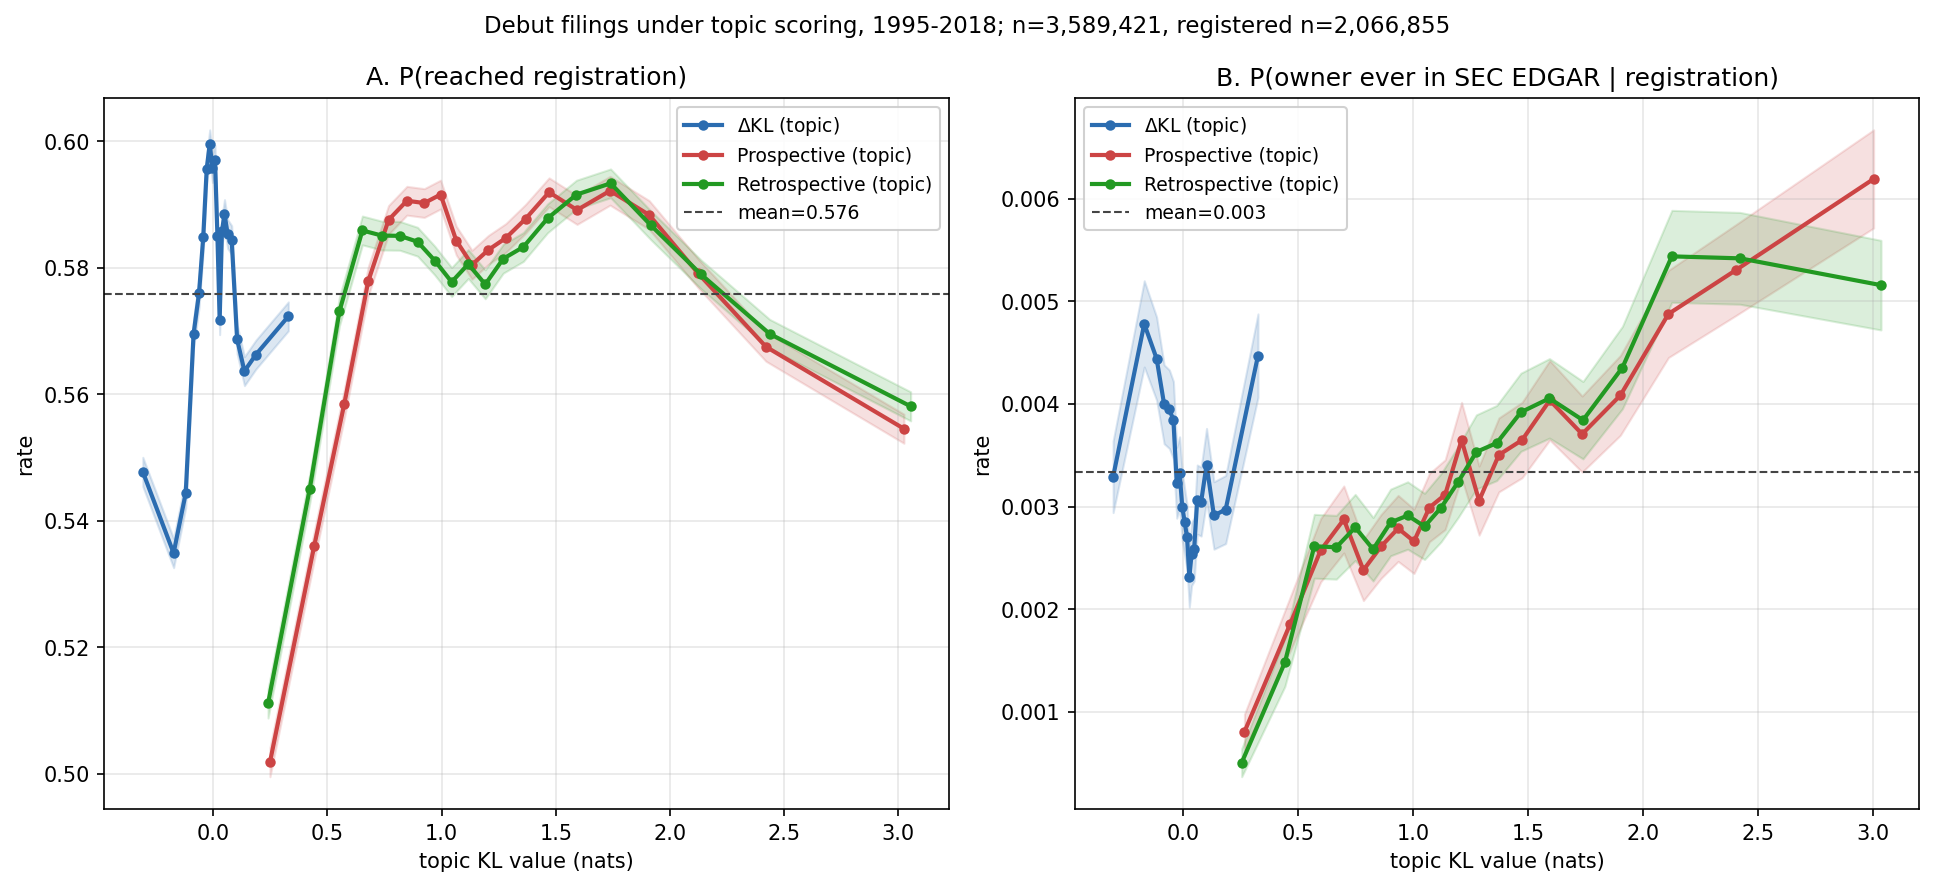
\includegraphics[width=\textwidth]{results/debut_outcome_topic.png}
\caption{Outcomes for debut filings (owner's first-ever filing) across all
45 Nice classes under topic scoring, filing years 1995--2018, in quantile
bins with 95\% intervals. $n = 3{,}589{,}068$; registered subset
$n = 2{,}066{,}600$. \emph{A:} P(reached registration). \emph{B:} P(owner
ever in SEC EDGAR, the Commission's public filing system $\mid$
registration); the structure in panel B is
decomposed in Section~\ref{sec:bluesea}.}
\label{fig:outcomes}
\end{figure}

\begin{figure}[h]\centering
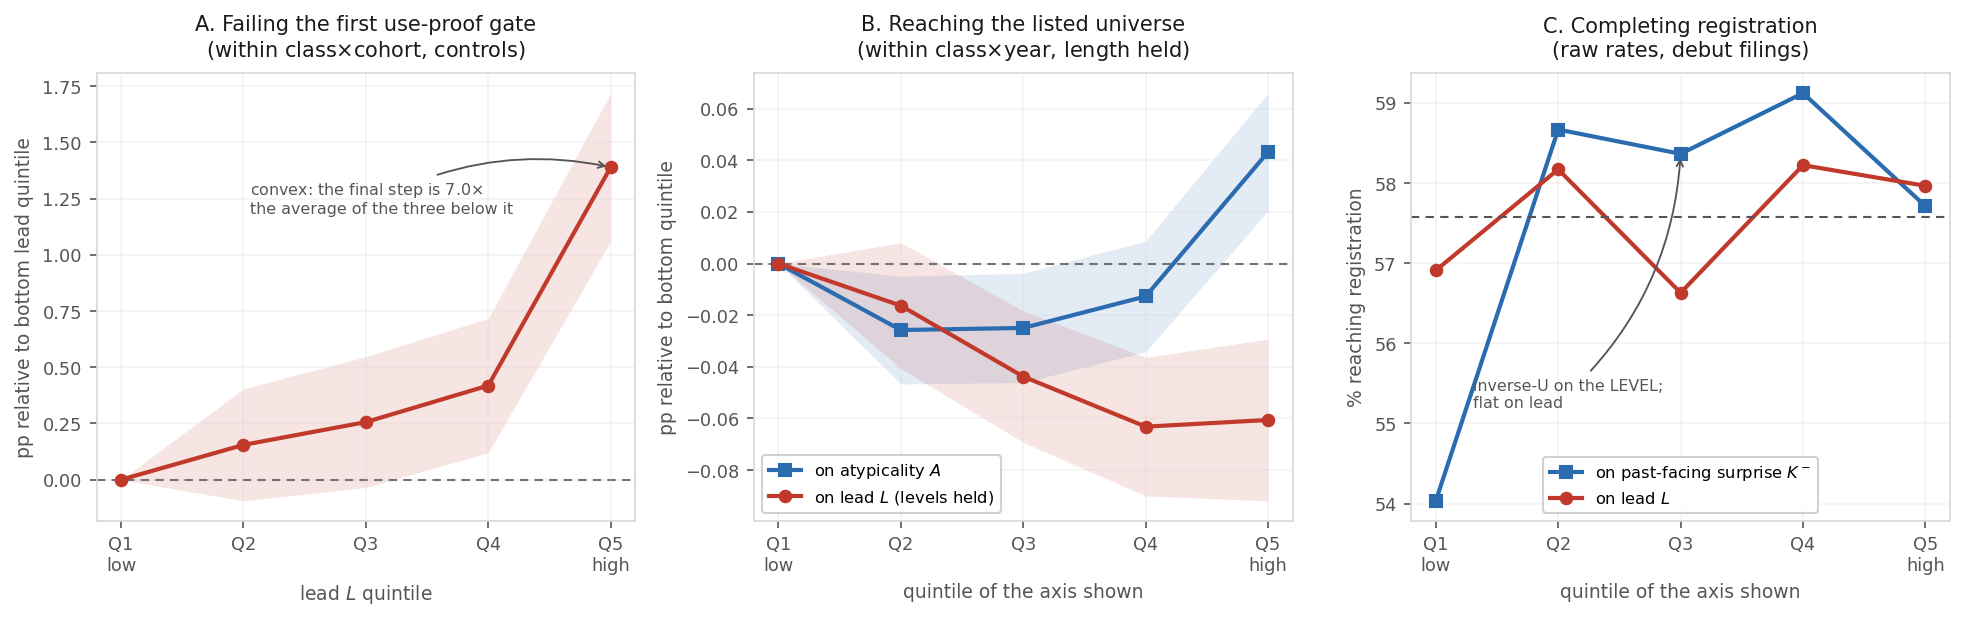
\includegraphics[width=\textwidth]{results/quintile_profiles.png}
\caption{Quintile profiles for the three outcomes. \emph{A:} the share of
registrations failing the first use-proof gate, by lead quintile, adjusted
within Nice class and registration year with the drafting and filer controls
of Table~\ref{tab:gate_lpm}; the dashed line is the rate for all
registrations. The profile rises gently and monotonically through the fourth
quintile and then steps up: about seven tenths of the top-to-bottom gap is
the single step from the fourth quintile to the fifth, seven times the
average step below it. A gradient is present, but the step at the top
dominates it, and the text reports top-versus-bottom contrasts for that
reason. \emph{B:}
the share of first-time filers whose owner ever reaches SEC reporting, by
quintile of atypicality and of lead, adjusted within Nice class and filing
year with description length held; flat in atypicality, and falling in lead
through the fourth quintile once the levels are controlled. Whiskers in A and
B are 95\% intervals on the difference from the bottom quintile. \emph{C:}
raw registration rates for debut filings in twenty bins --- an inverse-U on
atypicality, and on lead a trough just above the median that is
compositional, absent once atypicality is held in its middle fifth (dashed).
Horizontal line at the pooled rate.}
\label{fig:profiles}
\end{figure}

\subsection{Leading marks fail the use-proof gate}\label{sec:gate}

Marks written in language their industry subsequently moved toward fail
their first use-proof gate more often than marks written in language it was
moving away from. Within Nice class and registration year, controlling for whether the
filer drafted the mark themselves or hired counsel, and for the length of the
description, marks whose language most leads their industry fail $1.4$
points more often (53.3\%) than those in the most lagging fifth (51.9\%;
$t = 8.3$, Table~\ref{tab:gate_lpm}).

Among 4.12 million registration class-records 2002--2018, dated first-gate cancellation rises from 50.0\%
at the bottom topic-\dkl{} quintile to 52.4\% at the top, positive in 33
of 44 classes with sufficient volume (Figure~\ref{fig:forest}). But a raw
pooled contrast mixes the within-industry gradient with class and registration-year
composition, treats multi-class registrations as independent observations,
and ignores that gate outcomes correlate within owner. The
primary estimates therefore come from a linear probability model on 3.10
million unique registrations, one row per serial, with \dkl{} quintiles cut
\emph{within} Nice class and registration year. The specification adds
class$\times$registration-year fixed effects; controls for counsel of record,
intent-to-use basis, log description length, log owner filing volume, owner
domicile, and foreign filing basis;\footnote{A US application is filed
either on \emph{use} --- the mark is already in commerce --- or on
\emph{intent to use}, which defers proof until after allowance. Foreign
applicants may instead file on a home registration (\S44(e)) or extend an
international registration into the US under the Madrid Protocol
(\S66(a)); the latter maintain under \S71 rather than \S8. These are
statutory routes to the same registration, and they differ sharply in who
files and how often the mark is abandoned, which is why each enters as a
control.} and standard errors clustered on 1.27
million normalized owners (Table~\ref{tab:gate_lpm}).\footnote{Ties are
common. Within the class$\times$registration-year cell the quintiles are cut in,
$17.1$\% of scored registrations share a \dkl{} value with at least one
other filing, and the largest tie group runs to 53. Anchoring the reference
window on the filing date does not remove them, because filings that share a
class, a filing date and a goods/services description --- an owner
registering a family of marks at once, on Manual language --- have identical
distributions scored against identical references. Cut points are fixed by
sorting on the score and then on the serial number, which is reproducible
but systematic: serials run in filing order. It makes no difference. Sorting
the ties the opposite way moves the top-versus-bottom contrast by $0.001$pp,
and five pseudorandom orderings move it by at most $0.002$pp, against a
contrast of $2.287$pp --- a tenth of one percent of the estimate.}

\begin{table}[h]\centering\small
\caption{First-gate failure and \dkl{}: design-based estimates.
LPM of event-dated first-gate failure on within-class$\times$registration-year
\dkl{} quintiles (Q1 omitted), unique serials, registrations 2002--2018.
Failure is a dated cancellation for non-use at registration age 4.0--8.5
years, under \S8 or, for Madrid \S66(a) registrations, \S71.
All specifications include class$\times$registration-year fixed effects; controls
are counsel of record, intent-to-use basis, log goods/services length,
log owner filing count, owner domicile (US, CN), and foreign basis
(\S44(e), \S66(a)). Base failure rate 52.3\% on this sample.}
\label{tab:gate_lpm}
\begin{tabular}{llrrr}
\toprule
Sample & Specification & Q5$-$Q1 (pp) & SE & $n$ \\
\midrule
All & FE only & $+2.29$ & $0.16$ & 3{,}104{,}534 \\
All & FE + controls & $+1.39$ & $0.17$ & 3{,}104{,}534 \\
Counsel-represented & FE + controls & $+1.15$ & $0.20$ & 2{,}414{,}318 \\
Counsel + US-domiciled & FE + controls & $+1.60$ & $0.22$ & 1{,}888{,}352 \\
Self-filed & FE + controls & $+1.80$ & $0.26$ & 690{,}216 \\
Excluding Madrid \S66(a) & FE + controls & $+1.82$ & $0.18$ & 2{,}924{,}427 \\
\midrule
Counsel + US, 2002--07 & FE + controls & $-0.25$ & $0.33$ & 551{,}989 \\
Counsel + US, 2008--12 & FE + controls & $+2.00$ & $0.42$ & 551{,}924 \\
Counsel + US, 2013--18 & FE + controls & $+2.65$ & $0.25$ & 784{,}439 \\
\midrule
All & continuous, pp per sd of lead & $+0.58$ & $0.05$ & 3{,}104{,}534 \\
Counsel + US & continuous, pp per sd of lead & $+0.63$ & $0.06$ & 1{,}888{,}352 \\
\bottomrule
\end{tabular}
\\[0.3em]\footnotesize Standard errors replace significance stars: with $n$
in the millions every coefficient has $p < 0.01$, so stars would mark each
row identically. Errors are clustered on \emph{normalized owner} --- names
uppercased, stripped of punctuation and of twenty legal suffixes, so
\textsc{acme corp.} and \textsc{acme corporation} are one cluster. A single
owner files many marks, drafts them in a house style, and abandons them
together when the business fails; the within-owner correlation of gate
survival is $0.42$, so the 1.27 million owner clusters, not the filings,
carry the information. The Madrid row drops \S66(a) registrations rather
than absorbing them in a control, since they maintain under a different
statute; the estimate is larger without them.
\end{table}

The gradient is monotone within cells. Whether the filing was drafted by
counsel or by the owner is held because it moves both sides of the
comparison at once: self-filers fail the gate at 69.6\% against 46.8\% for
represented owners, and they write shorter descriptions that sit closer to
their class's usual language yet lean slightly further ahead of it, so
without the control, part of any lead gradient is a self-filing gradient. With it, the penalty is of the same order in both
strata ($+1.8$pp self-filed, $+1.2$pp counselled). The full control set cuts the
magnitude by about a third without absorbing it, and the estimate is if
anything \emph{largest} in the cleanest stratum --- counsel-represented,
US-domiciled owners --- so it is not carried by the self-filed or foreign
mass-filing segments whose gate failure rates are high for their own
reasons.\footnote{The level effects on those covariates are large in their
own right: counsel $-19.5$pp and Madrid \S66(a) basis $+10.3$pp.} About
forty percent of the raw pooled contrast is composition: $+1.4$pp
design-based against $+2.5$pp raw.

\begin{figure}[h]\centering
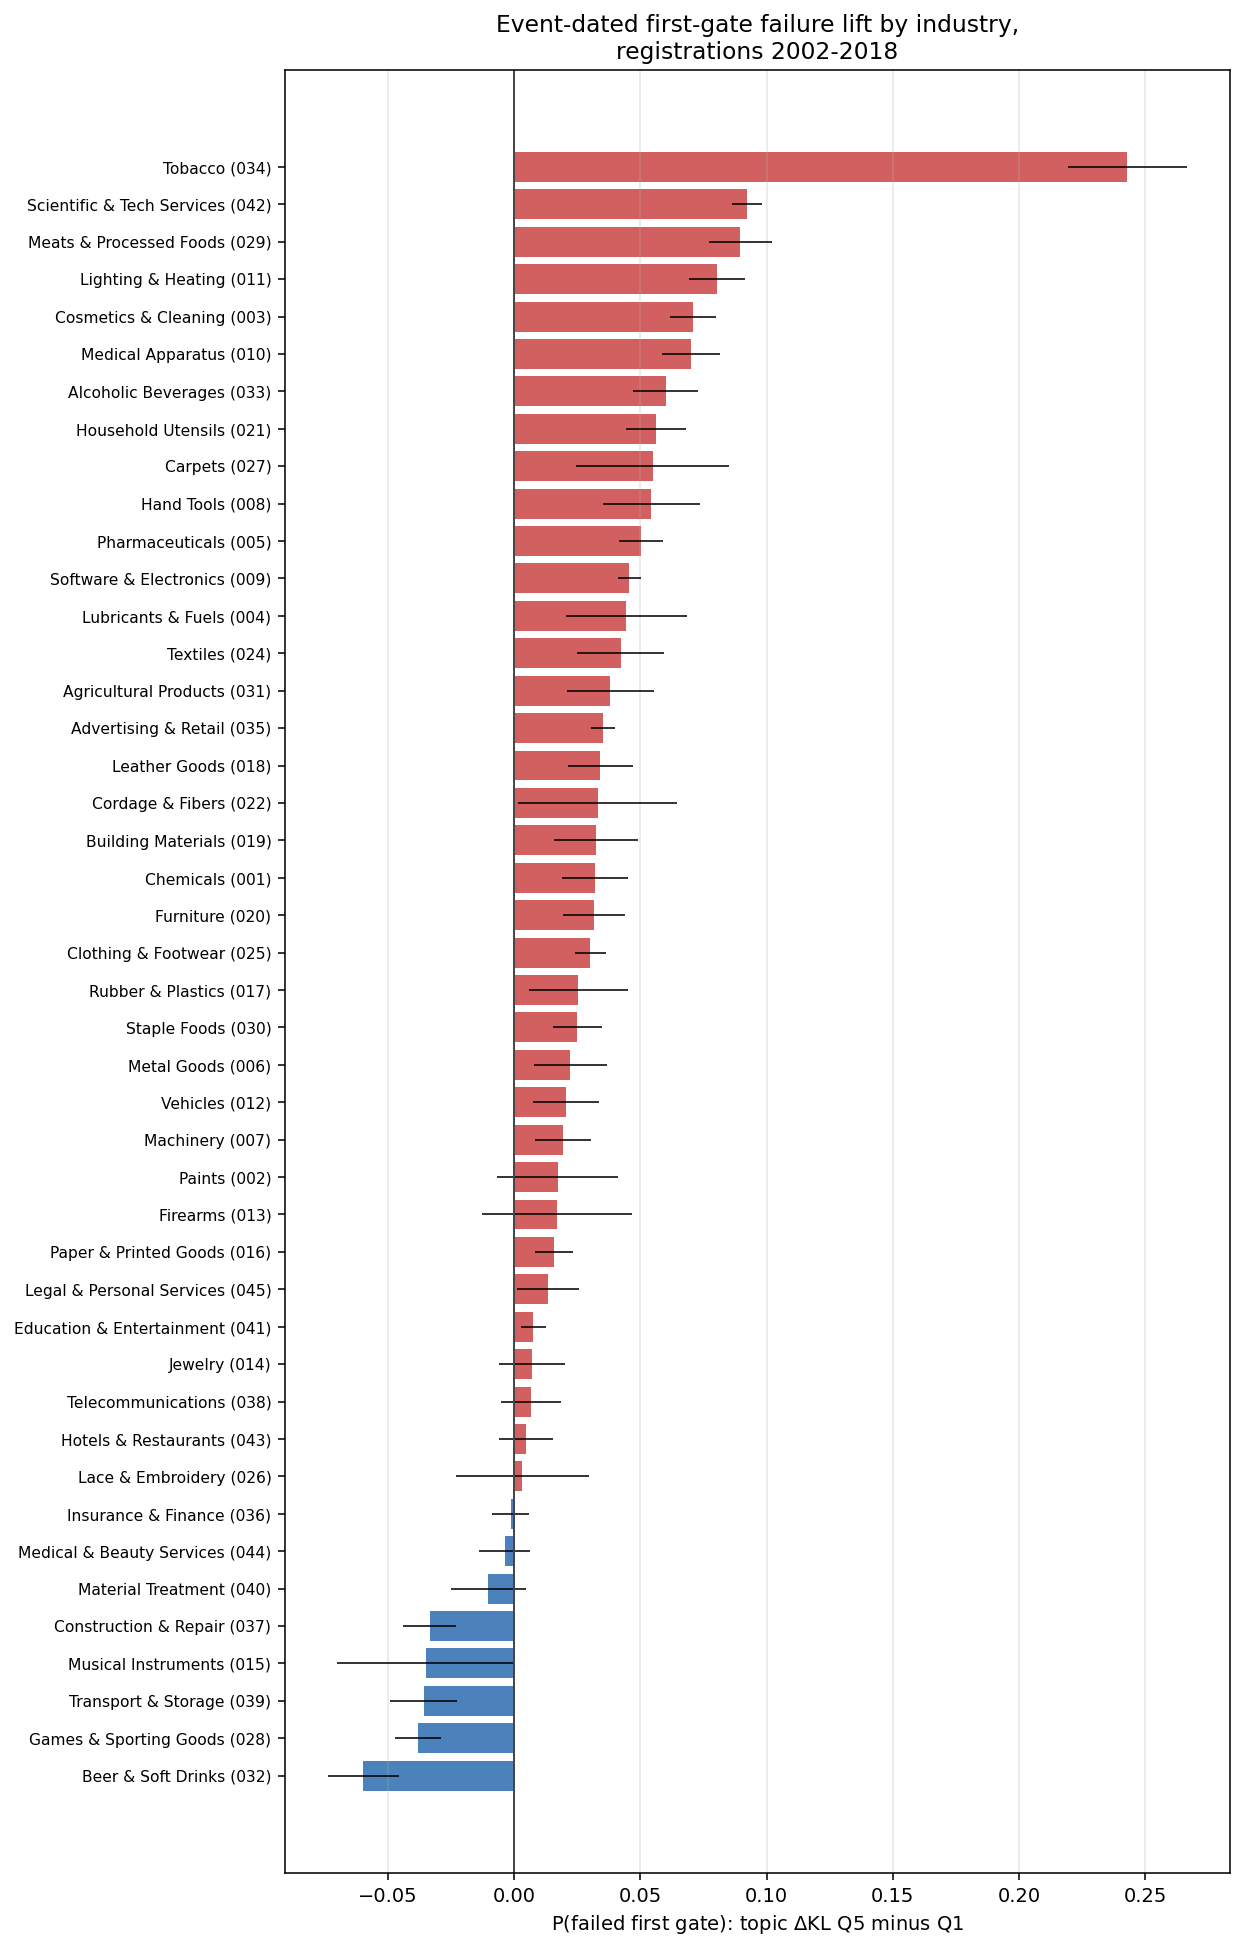
\includegraphics[width=0.72\textwidth]{results/event_gate_forest.png}
\caption{Event-dated first-gate failure lift (topic \dkl{} top minus
bottom quintile) by industry, registrations 2002--2018, raw quintile
contrasts. Positive bars indicate the leading penalty. Whiskers are
two-sample binomial intervals, uncorrected for the within-owner correlation
($0.42$) and so narrower than clustered intervals; read
Table~\ref{tab:gate_lpm} for precision. Per-class breakouts are in the
online appendix.}
\label{fig:forest}
\end{figure}

Within the 2002--2018 window the penalty looks modern: indistinguishable
from zero for the 2002--2005 cohorts, turning positive in 2006, and running
$+1.8$ to $+5.6$pp for every cohort from 2008 onward
(Figure~\ref{fig:cohort}). That reading does not survive carrying the
series back: the penalty was two to three times larger for the earliest
scoreable cohorts than for any since, which makes the 2002--2005 quiet a trough
between two episodes rather than a starting point (Section~\ref{sec:eras}).

The gate is close to a fixed appointment rather than a hazard spread over years: of the 1.35 million
cancellations recorded for fully observed cohorts, 17 post before
registration age 6.5, 96.1\% post between 6.5 and 7.0, and the rest after
seven. Since the cancellation record ends on 2 April 2026, a cohort is
observable only once it has reached seven years, which makes 2019 the last
one with usable gate data and leaves 2020 and later with no observed gate at
all. Measured on the 6.5--7.0 band, fully observed for every cohort it
covers, the penalty runs between $+2.1$ and $+5.6$pp with no trend across
the decade and overlapping intervals at its two highest points. The 2019
reading rests on the 78{,}408 registrations issued early enough in that year
to reach seven years inside the record, so it is a first-quarter subsample
rather than a cohort.

The outcome is an indicator on a window, so a mark that fails outside it
counts as a survivor. If leading marks failed at the same rate as lagging ones
but sooner, that alone would put them inside the window more often and the
measure would report a difference in rates where there was only a difference in
timing. It is not.
On the 3.15 million registrations whose ninth anniversary is inside the
record --- for which failure is settled and no window is needed --- the
contrast is $+2.71$pp within class and registration year, against $+2.65$pp on the
paper's 4.0--8.5 window and $+2.65$pp on the narrow band. Conditional on failing, the probability of failing late
carries a contrast of $-0.01$pp ($t = -0.2$) once class and registration year are
held. The pooled version of that contrast is $+0.27$pp and is composition.

The filer population changed over the same period. Within
counsel-represented US-domiciled owners, and with the full control set, the
earliest cohort third is slightly negative ($-0.25$pp, SE $0.33$) while the
two later thirds are clearly positive ($+2.00$ and $+2.65$pp,
Table~\ref{tab:gate_lpm}). The gradient is therefore not an artefact of the
post-2015 surge in self-filed and foreign applications.

\begin{figure}[h]\centering
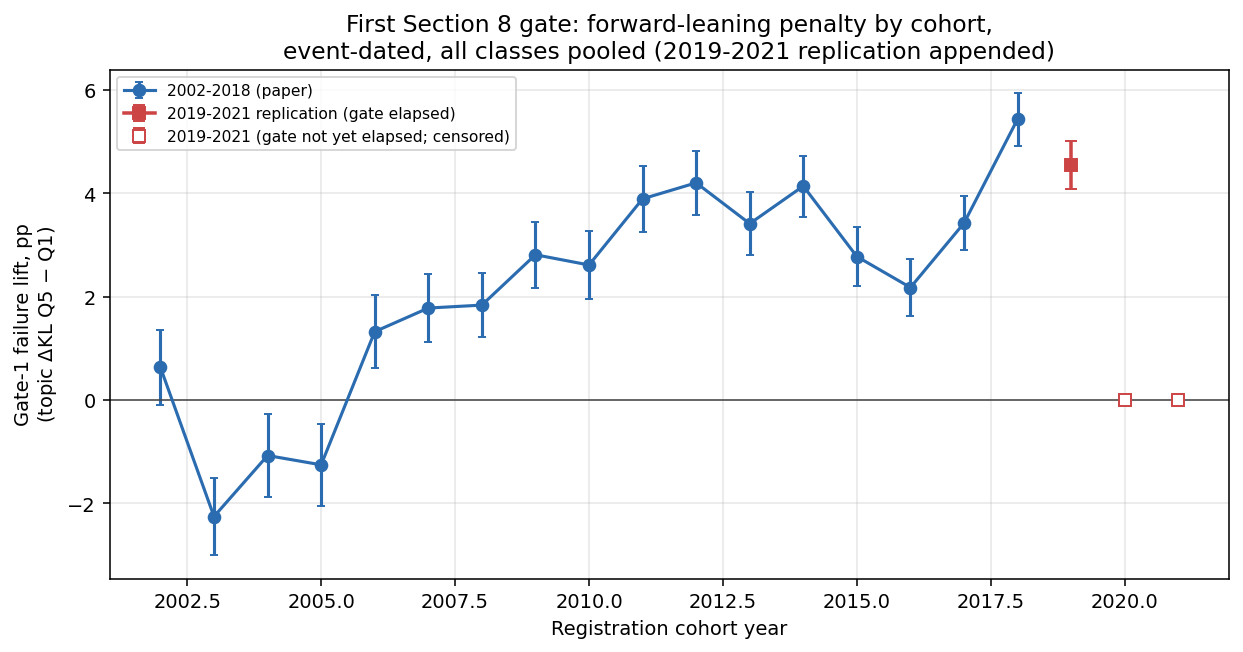
\includegraphics[width=0.8\textwidth]{results/event_gate_cohort_curve_extended.png}
\caption{The leading gate penalty by registration cohort, all classes
pooled. Each point is the event-dated first-gate failure rate of the most
leading fifth of that cohort's registrations minus that of the most lagging
fifth, with lead quintiles cut within the cohort and no controls. The penalty is
absent or negative for the 2002--2005 cohorts, turns positive in 2006, and
is present in every cohort from 2008 through 2019, ranging $+1.8$ to
$+5.6$pp with no downward trend. 2019 is the last evaluable cohort:
cancellations post at about age six and a half and the record ends in April
2026, so later cohorts have not reached their gate rather than having
passed it.}
\label{fig:cohort}
\end{figure}

\subsection{The penalty is not modern, and it is not general}\label{sec:eras}

Scores exist from 1995 on, which makes registration cohorts from 1996 evaluable, and their gate
outcomes have been settled for two decades. Carried back, the contrast runs
$+6.9$pp for the 1996 cohort and rises to $+10.1$pp for 1999 --- two to
three times anything observed since --- then collapses. The 2002--2005
cohorts the paper had been reading as a quiet baseline are a trough between
two episodes, and one of them is the larger.

Scores begin in 1995, so a 1996-cohort registration must have issued within
a year of filing; early cohorts are selected on prosecution speed, and speed
plausibly travels with drafting in standard language. Holding pendency in a
common one-to-three-year band leaves the series unchanged. Indexing by
filing year instead, so a cohort contains every prosecution speed, gives
$+7.9$ to $+9.6$pp for filings 1995--1999 and $-0.95$pp for filings made in
2000 --- a ten-point swing in a single filing year.

Splitting the four classes that carry most technology filings --- 009, 035, 038 and 042 ---
against the other forty-one separates a large moving component from a small
steady one (Figure~\ref{fig:eras}):

\begin{center}\small
\begin{tabular}{lrr}
\toprule
Filing years & Technology classes & All others \\
\midrule
1995--1999 & $+14.18$ (0.36) & $+4.48$ (0.27) \\
2000--2004 & $-1.37$ (0.35) & $+1.21$ (0.24) \\
2005--2007 & $+2.04$ (0.43) & $+1.99$ (0.28) \\
2008--2014 & $+9.02$ (0.25) & $+1.32$ (0.17) \\
\bottomrule
\end{tabular}
\end{center}

\noindent Outside technology the penalty is a flat $+1$ to $+4$pp in every
era, including the one in which the pooled series reads as zero. Inside
technology it swings by fifteen points: strongly positive for filings made
into the late 1990s, negative for those made in the five years after, and
positive again from 2008. The pooled null of 2002--2005 is a technology
reversal partly offsetting a non-technology positive, not an absence.

What this design cannot say is which cycle the swing belongs to. Marks filed
1995--1999 reach their gate in 2001--2007 and marks filed 2000--2004 reach
theirs in 2006--2013, so a story in which unusual language is punished
because it was written during an investment boom and a story in which it is
punished because the gate falls during a bust both fit these numbers.

\begin{figure}[h]\centering
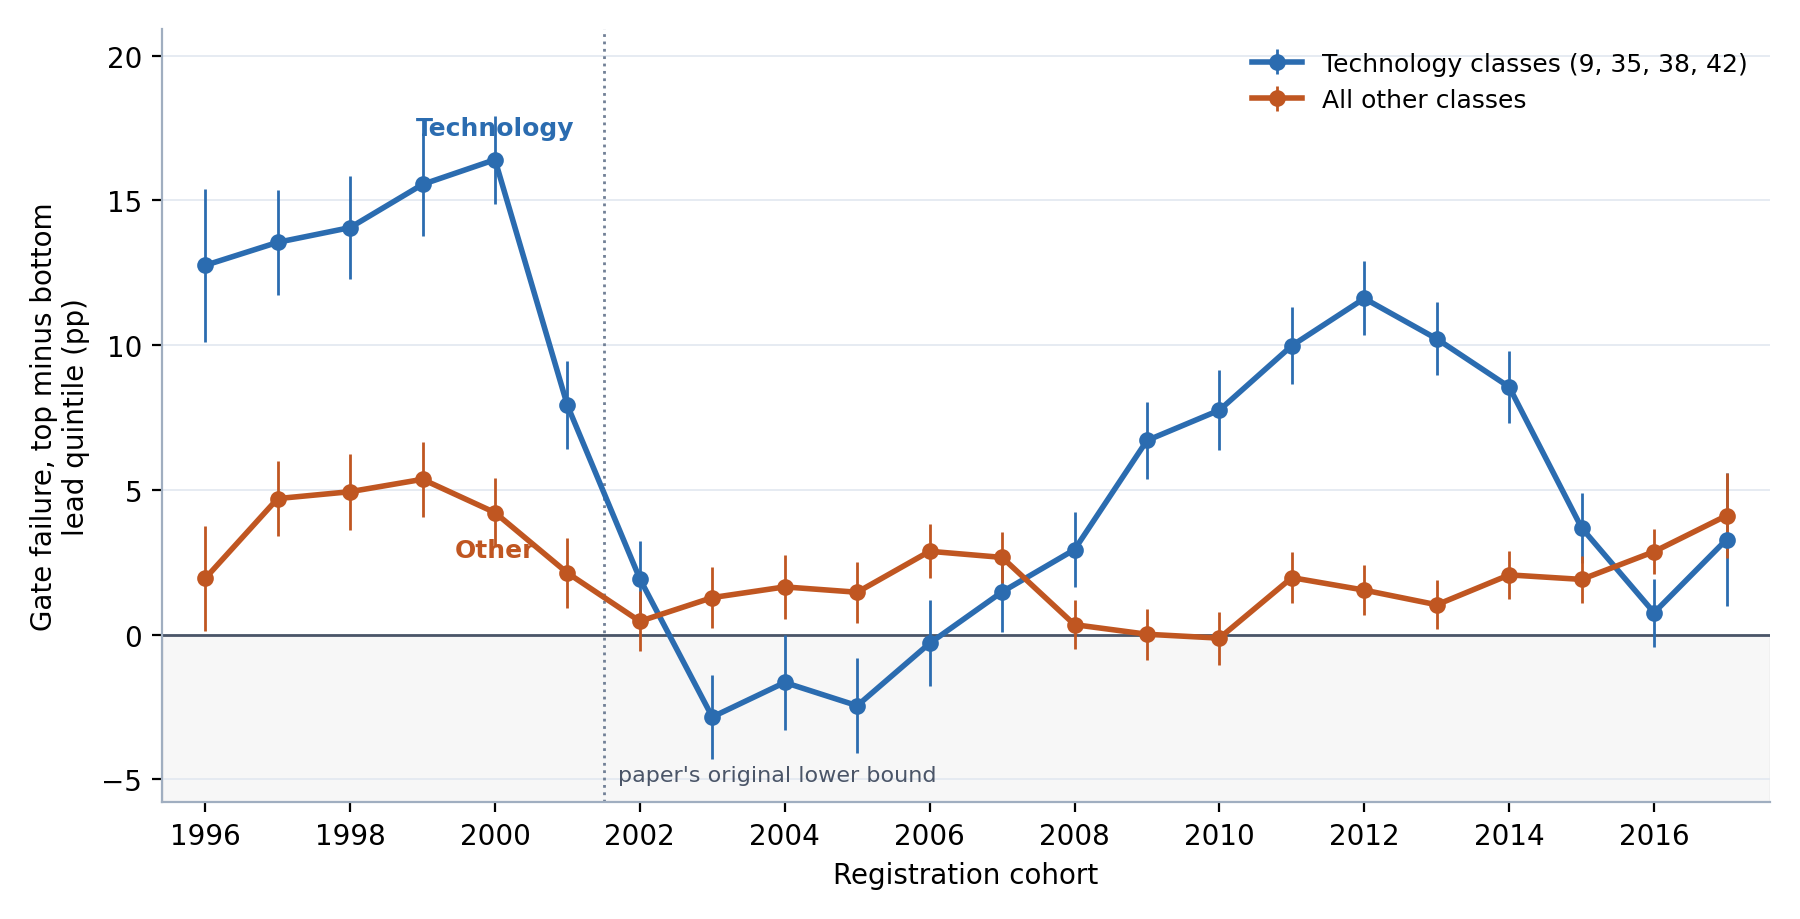
\includegraphics[width=0.86\textwidth]{results/gate_era_profile.png}
\caption{The leading gate penalty by registration cohort, technology classes
(009, 035, 038, 042) against all others. Each point is the first-gate failure
rate of the most leading fifth of that cohort's registrations minus that of the
most lagging fifth, lead quintiles cut within cohort and group, no controls,
with 95\% intervals. Cohorts are
restricted to registrations whose ninth anniversary is inside the record, so
every outcome shown is settled. Outside technology the penalty is small and
almost flat across two decades; inside technology it swings from $+16$pp for
the 2000 cohort to $-3$pp for 2003 and back to $+12$pp for 2012. The dotted
line marks the 2002 cut that the main cohort series uses.}
\label{fig:eras}
\end{figure}

\subsection{Three of the four classes reverse, and the leading language changes theme}\label{sec:techswing}

The four-class split pools industries that do not move together. Taking
them one at a time, and then assigning quintiles inside progressively finer
cells (Table~\ref{tab:techswing}):

\begin{table}[h]\centering\small
\caption{The leading gate penalty inside technology, by class and by cell.
Top-minus-bottom lead-quintile contrast in first-gate failure (pp, SE in
parentheses), settled registrations, by filing era. The upper block assigns
quintiles within each class and era. The lower block pools the four classes
and assigns quintiles within the era (raw, as in the text table above),
within class$\times$registration-cohort cells, and within
theme$\times$class$\times$registration-year cells, where a filing's theme is the one
its description loads most heavily on under the production $T = 50$ model.
$n = 1{,}248{,}591$.}
\label{tab:techswing}
\begin{tabular}{lrrrr}
\toprule
Class & 1995-1999 & 2000-2004 & 2005-2007 & 2008-2014 \\
\midrule
009 Electrical, software & $+18.04$ (0.52) & $-5.32$ (0.51) & $+0.25$ (0.62) & $+11.67$ (0.37) \\
035 Business services & $+4.59$ (0.69) & $-9.70$ (0.56) & $+2.02$ (0.63) & $+1.66$ (0.36) \\
038 Telecommunications & $+9.91$ (1.40) & $-4.24$ (1.29) & $+2.60$ (1.48) & $+3.42$ (0.94) \\
042 Scientific, computer services & $+17.11$ (0.57) & $+6.70$ (0.62) & $+8.42$ (0.87) & $+12.63$ (0.47) \\
\midrule
Four classes pooled, raw & $+14.49$ (0.33) & $-1.81$ (0.31) & $+2.56$ (0.38) & $+9.16$ (0.22) \\
\quad within class$\times$cohort & $+14.27$ (0.33) & $-3.63$ (0.31) & $+2.73$ (0.38) & $+7.24$ (0.22) \\
\quad within theme$\times$class$\times$cohort & $+4.78$ (0.33) & $-1.26$ (0.31) & $+2.56$ (0.38) & $+4.51$ (0.22) \\
\bottomrule
\end{tabular}

\end{table}

\noindent Electrical and software goods (009) and telecommunications (038)
follow the pooled pattern. Business services (035), the class that holds
online retail, reverses hardest: $-9.7$pp for filings made 2000--2004 against
$+4.6$pp in the five years before. Scientific and computer services (042)
never reverses. Its contrast is $+6.7$pp in the era in which the other three
are negative and between $+8$ and $+17$pp in every other, and by registration
cohort it never falls below $+3$pp (Figure~\ref{fig:techswing}). The
reversal is an event in goods and in business services; the class that
sells technology as a service sat it out.

Assigning quintiles within class and registration year rather than within the era
pool changes little. Assigning them within theme, class and registration year
changes a great deal: the late-1990s contrast falls from $+14.5$ to
$+4.8$pp, the post-2008 contrast from $+9.2$ to $+4.5$pp, and the 2000--2004
reversal from $-3.6$ to $-1.3$pp. Two thirds of the first and half of the
second are between themes rather than within them. The leading fifth of each
era was drawn from particular themes, and those themes carried their own
failure rates; the penalty for being leading \emph{inside} a theme is a
steadier $+2.5$ to $+5$pp, the same order as the penalty outside technology.

Which themes is a matter of record (Table~\ref{tab:techthemes}). In
1995--1999 the computer, software, information and data services theme held
38\% of technology filings and 75\% of the leading fifth, and its
registrations failed at 58.9\% against 46--53\% in the other large themes.
That one theme is most of the late-1990s penalty. In 2000--2004 it held
12\% of the leading fifth. The leading language had moved to video, music
and games on electronic media (31\% of the leading fifth against 12\% of
filings) and the internet-services language had become lagging --- wording
the class was leaving --- and inside several themes the lagging fifth now
failed more than the leading one: $-3.6$pp in electronic media, $-5.5$ in
retail store services, $-6.9$ in apparatus and control systems. From 2008
the leading fifth over-represents downloadable and online software by four
to one (15\% against 4\%), the vocabulary of the application store; those
registrations fail at 67.2\%, the highest base rate of any theme, and carry
the largest within-theme contrast anywhere in the table, $+8.4$pp. The
computer-services theme's own contrast, meanwhile, is positive in every era
($+3.6$ to $+5.9$pp) and never reverses.

\begin{table}[h]\centering\footnotesize
\caption{The leading gate penalty by theme within the four technology
classes. Themes with at least 20{,}000 settled registrations, labelled by
their five highest-probability terms; quintiles assigned within theme and
era. Cells with fewer than 3{,}000 registrations are blank.}
\label{tab:techthemes}
\begin{tabular}{p{5.2cm}rrrrr}
\toprule
Theme (top words) & $n$ & 1995-1999 & 2000-2004 & 2005-2007 & 2008-2014 \\
\midrule
services, computer, software, information, data & 451,253 & $+3.61$ (0.52) & $+3.56$ (0.49) & $+4.18$ (0.64) & $+5.92$ (0.37) \\
video, computer, electronic, music, games & 162,290 & $+2.53$ (0.97) & $-3.62$ (0.89) & $-2.85$ (1.01) & $+3.36$ (0.60) \\
services, featuring, store, retail, store services & 131,107 & $+8.39$ (1.09) & $-5.49$ (1.01) & $+2.92$ (1.15) & $+0.98$ (0.66) \\
services, field, training, estate, educational & 95,602 & $+7.82$ (1.09) & $+0.99$ (1.12) & $+6.02$ (1.43) & $+2.05$ (0.83) \\
apparatus, systems, devices, electronic, control & 84,121 & $+4.80$ (1.27) & $-6.92$ (1.19) & $-0.58$ (1.41) & $+3.65$ (0.88) \\
design, field, systems, development, services & 32,517 & $+10.40$ (2.03) & $+4.67$ (1.82) & $+1.50$ (2.27) & $-2.27$ (1.45) \\
software, online, downloadable, non-downloadable, virtual & 29,472 & --- & --- & --- & $+3.30$ (1.05) \\
bags, clothing, shirts, jackets, leather & 28,421 & $+1.28$ (2.59) & $-1.55$ (2.39) & $-4.66$ (2.40) & $+6.06$ (1.36) \\
research, medical, scientific, testing, purposes & 25,897 & $+12.65$ (2.66) & $+12.09$ (2.03) & $-3.82$ (2.59) & $+5.63$ (1.51) \\
services, health, field, care, information & 22,880 & $+4.94$ (2.04) & $+1.39$ (2.36) & --- & $+3.50$ (1.72) \\
\midrule
All themes, within theme$\times$class$\times$cohort & 1,150,921 & $+4.78$ (0.33) & $-1.26$ (0.31) & $+2.56$ (0.38) & $+4.51$ (0.22) \\
\bottomrule
\end{tabular}

\end{table}

\begin{figure}[h]\centering
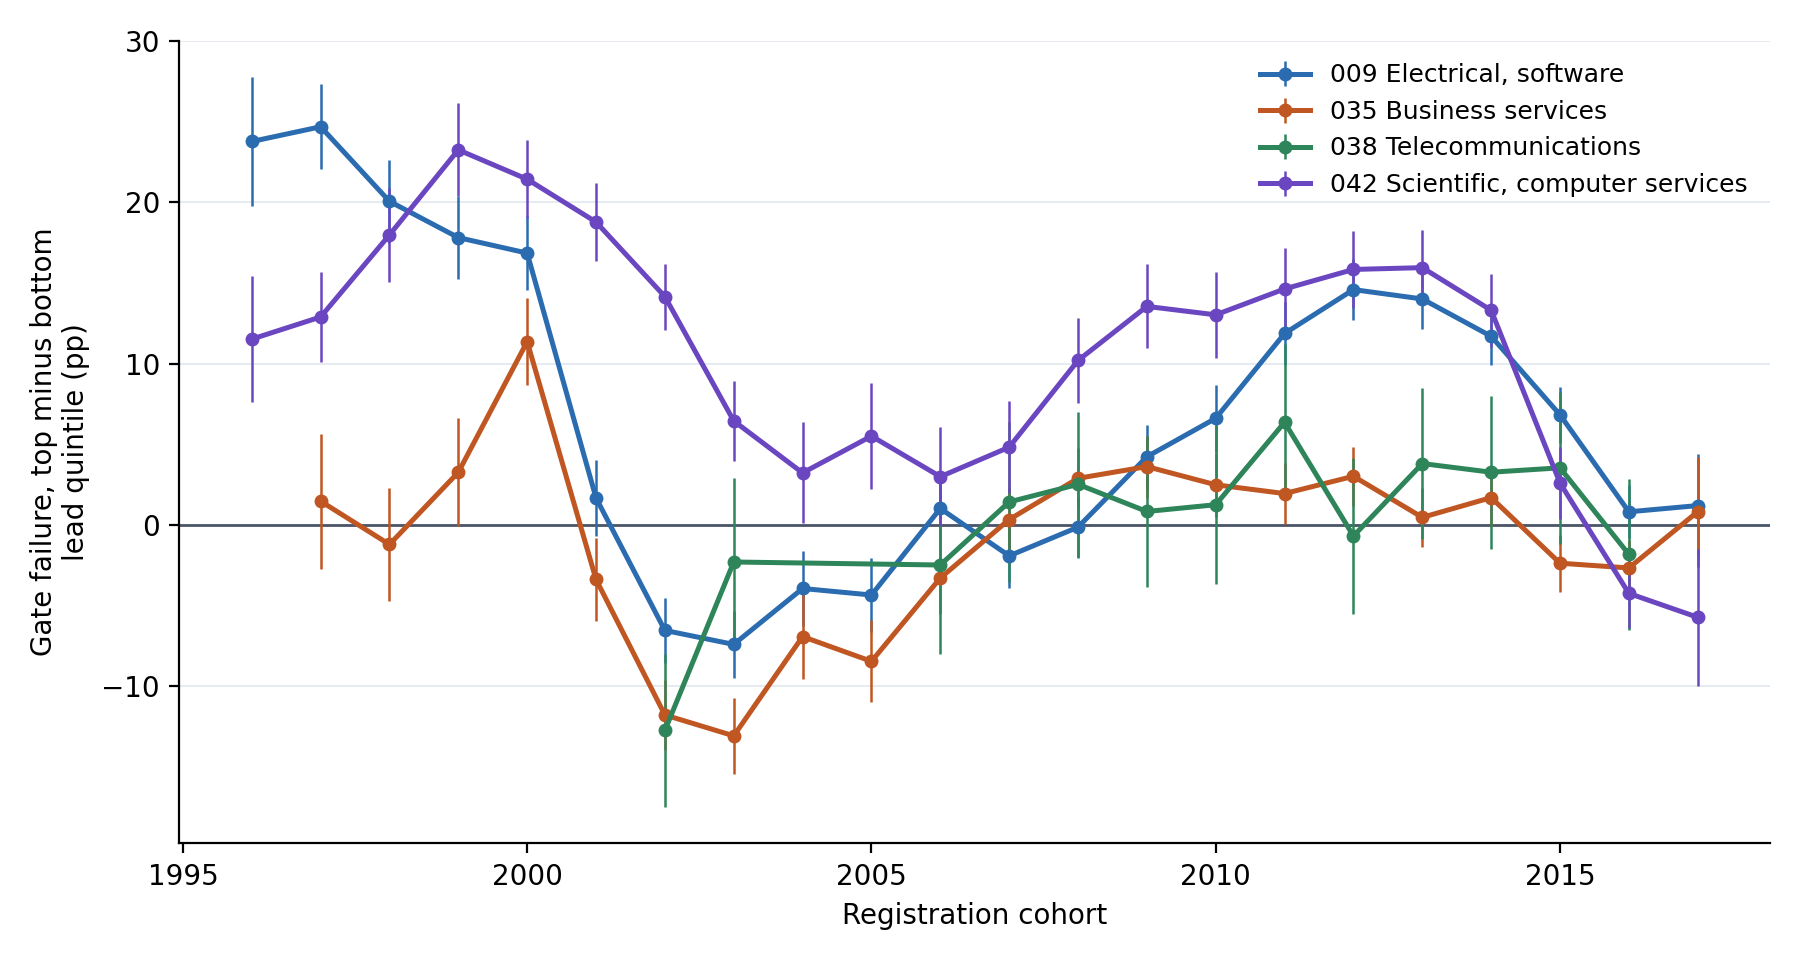
\includegraphics[width=0.92\textwidth]{results/gate_era_tech_themes.png}
\caption{The leading gate penalty by registration cohort, one line per
technology class. Each point is the first-gate failure rate of the most
leading fifth of that class and cohort's registrations minus that of the most
lagging fifth --- lead quintiles cut within class and cohort, no controls ---
with 95\% intervals, on registrations whose gate outcome is settled. Three
classes cross zero between 2001 and 2006; scientific and computer services
does not.}
\label{fig:techswing}
\end{figure}

So the swing has two layers. Across the whole period, a leading filing is a
few points more likely to fail than a lagging one in the same theme, class
and cohort, in technology as elsewhere. On top of that, each era's leading
vocabulary was concentrated in one or two themes whose marks failed at
their own rate: internet services in the 1990s, application software after
2008. In the trough between, the language that had been leading became
lagging, and the marks still written in it failed with it. The
design-based estimates in Table~\ref{tab:gate_lpm} hold class and cohort
fixed but not theme, so they carry both layers; a reader who wants only the
within-theme penalty should take the lower block of Table~\ref{tab:techswing}
as the guide to its size.

Levels and gradients separate cleanly across filer strata. Self-filers
fail the gate far more often than represented owners (69.6\% versus
46.8\%), and intent-to-use registrations more often than use-based ones
(53.1\% versus 50.2\%),
but the \dkl{} gradient itself is similar across these strata once class,
cohort, and drafting covariates are held fixed ($+1.8$pp self versus
$+1.2$pp counseled in Table~\ref{tab:gate_lpm}). Per class, the largest penalties sit in tobacco ($+26$pp, the
vaping era), hand tools ($+10$pp), processed foods ($+10$pp) and medical
apparatus ($+9$pp), with negative lifts in beverages, transport and
construction.

The risk persists at the year-ten renewal, and on the design-based
estimates does not attenuate: the lead coefficient is $-0.49$pp at the first
gate and $-0.63$pp at the second (Table~\ref{tab:staged}). What attenuates is
the raw single-class contrast. In the
software diagnostic class, where the event-dated first-gate lift on the
2010--2013 cohorts reaches $+12.1$pp, the conditional lift at the second
gate falls to $+7.6$pp. Pooled across classes the second-gate profile is not
a slope at all. Fitted over 872{,}079 first-gate survivors with a resolved
year-ten status, a straight line through renewal against lead explains 1\% of
the variation across forty bins and a V explains 89\%
($\Delta$AIC $= 83$, the largest margin anywhere in this paper). Renewal is
highest at both ends of the lead axis and lowest just below its centre. The
$-0.63$pp linear coefficient reported for that row is therefore close to
meaningless as a description, though it is not wrong about the direction of the
leading tail. By year ten the lagging tail has closed the gap in cumulative
failure, having simply taken longer to get there. Most of the difference
resolves at first proof of use.

A competing reading is that the gate measures disengagement rather than
products: an owner who has lost interest both answers the examiner slowly
and lets the registration lapse. The prosecution record tests this through
the gap between the first non-final office action and the response to it.

Response speed does not predict the gate. Across the 1.22 million scored
registrations with a usable office-action/response pair, gate passage varies
between 46.1\% and 48.1\% across response-speed quintiles, from a median of
seven days to 183 --- flat, and if anything the quickest responders pass
slightly \emph{less}. The lead penalty is present in both halves: $-3.48$pp
($\pm 0.40$) among faster-than-median responders and $-2.36$pp ($\pm 0.40$)
among slower, against $-2.94$pp pooled. The restriction drops 61\% of
the sample, disproportionately applications that never drew a refusal, so
this speaks to the prosecuted subset.

Mixing the past and future reference windows identifies which kind of
novelty the gate punishes. Scored against a long past and a short future,
so that lead measures a break with what the class had established, the
top-versus-bottom contrast is $+3.0$pp; scored against a short past and a
long future, so that it measures resemblance to where the class was
heading, it is $+1.65$pp. The symmetric five-year measure sits between, and
the penalty rises monotonically along the mix. The gate punishes breaking
with the past more than it punishes anticipating the future, but it
punishes both (Appendix~\ref{app:comp}).

\subsection{Being early costs at the public-reporting margin; being unusual does not pay there}\label{sec:bluesea}

The outcome here is whether an owner ever appears in the Securities and
Exchange Commission's financial reporting records. That is broader than
exchange-listed: roughly half the matched firms carry a ticker and the rest
report for other reasons. The rate rises monotonically in
the KL \emph{levels} on both axes, from 0.19\% at the bottom past-facing
quintile to 0.52\% at the top. In signed \dkl{} it is U-shaped.

\begin{table}[h]\centering\small
\caption{Debut listing and vocabulary position: design-based estimates.
LPM of P(owner ever in SEC EDGAR) on 1{,}556{,}968 registered debut
filings 1995--2018, one observation per owner, class$\times$filing-year
fixed effects, heteroskedasticity-robust SEs. Quintiles cut within
class$\times$year. Base rate 0.481\%.}
\label{tab:edgar}
\begin{tabular}{lrr}
\toprule
 & Coefficient (pp) & SE \\
\midrule
\multicolumn{3}{l}{\emph{Atypicality quintiles, $A = \tfrac{1}{2}(K^{-}+K^{+})$ (Q1 omitted)}} \\
\quad Q5, FE only & $+0.017$ & $0.018$ \\
\quad Q5, FE + log length & $+0.000$ & $0.018$ \\
\quad Q5, FE + log length, on $K^{-}$ alone & $-0.003$ & $0.018$ \\
\midrule
\multicolumn{3}{l}{\emph{Signed \dkl{} quintiles, FE + log length + KL levels}} \\
\quad Q3 & $-0.133$ & $0.020$ \\
\quad Q4 & $-0.187$ & $0.021$ \\
\quad Q5 & $-0.158$ & $0.024$ \\
\midrule
\multicolumn{3}{l}{\emph{Decomposition, FE + log length}} \\
\quad $|\Delta\mathrm{KL}|$ (pp per sd) & $+0.067$ & $0.009$ \\
\quad signed \dkl{} (pp per sd) & $-0.047$ & $0.006$ \\
\quad log description length & $+0.056$ & $0.004$ \\
\bottomrule
\end{tabular}
\\[0.3em]\footnotesize Standard errors in place of significance stars; see the
note to Table~\ref{tab:gate_lpm}.
\end{table}

The raw atypicality gradient does not survive the design-based estimates (Table~\ref{tab:edgar}). Within class and filing year, holding description length
fixed, top-quintile atypicality raises the probability of SEC reporting by
$+0.000$pp on a 0.481\% base ($t = 0.0$), and by $-0.003$pp on the past
level alone. The quintile profile is not even monotone: the three middle
quintiles sit \emph{below} the bottom one and the top merely returns to it.
The 2.7-fold gradient in the raw bins is composition --- firms that go on to
report cluster in particular classes, years, and multi-class filings --- and
class$\times$year fixed effects absorb it. Lead costs, at equal
atypicality: the signed component enters negatively
($-0.047$pp per standard deviation, $t = -7.8$) while the unsigned component enters
positively ($+0.067$pp per standard deviation, $t = 7.7$). The U-shape in raw bins
is exactly this pair: lagging filings show the atypicality premium with no
lead penalty, leading filings show it net of that penalty, and the middle
quintiles show neither. Once the levels are controlled,
the apparent recovery of the far-leading tail is much reduced: the quintile
profile falls through Q4 and recovers only slightly at Q5
(Table~\ref{tab:edgar} middle panel).

Owners are matched to SEC
registrants by normalized exact name, over a candidate universe of all
5.67 million owners in the corpus; names resolving to more than one
registrant are dropped rather than assigned, and one match is kept per owner
string. That yields 19{,}889 matched owners covering 7{,}588 registrants, and
a base rate of 0.481\% among registered debut filers. Validation on 22
companies that indisputably went public --- across software,
pharmaceuticals, food, apparel, aerospace and autos --- matches all 22. A random sample of 25 matches
carrying at least three filings was inspected by hand and none was wrong,
which is a check on gross failure modes rather than a precision estimate.

The linkage is nonetheless a name match, and that bounds the atypicality
reading in particular. Firms with distinctive names are easier to match than
firms with generic ones, and distinctiveness of a name plausibly travels with
distinctiveness of the goods/services text; nothing in this design separates
the two. Restricting the candidate universe --- to a subset of classes, say
--- makes matchability itself a function of the regressor, and the
atypicality gradient is sensitive to exactly that. Its absence here is
therefore the more credible reading of the two, and the signed axis, which
does not move when the linkage is varied, carries the weight. The financing
rows of Table~\ref{tab:staged} rest on a Form~D match whose raw extracts are
not in the current tree and should be read as provisional.

In raw rates, 0.444\% of the most
lagging fifth of registered debut owners later appear in SEC reporting
records, against 0.240\% in the middle fifth and 0.390\% of the most leading
fifth: both tails beat the middle, and the lagging tail beats the leading
one. Under the design-based specification the profile declines from the
lagging end through the fourth quintile and recovers slightly at the leading
end, so the ordering is monotone over four of the five quintiles.

The profile is a U rather than a slope, so a linear
summary of it points downward through a curve whose tails are its high
points; Appendix~\ref{app:choices} fits it: a V with its vertex about a
third of a standard deviation above mean lead, explaining 59\% of the binned
variation against 13\% for a straight line. And ``SEC reporting'' is
not ``went public'': splitting matched owners on whether their SEC filer number carries a
ticker gives $10{,}556$ listed against $9{,}333$ reporting without one, and
both halves show the same U, so the result is not an artifact of counting
non-operating registrants as successes.

Atypicality predicts survival at the use-proof gate but not which owners become SEC-reporting once composition is
absorbed. Lead is the timing bet, and it costs at both margins.

The two are not independent in the obvious economic sense. What makes a
filing leading is precisely that its industry moved toward its language, and
an industry that has moved toward your language now describes its goods the
way you describe yours. Being early therefore consumes the quantity that
pays: the mark that was unusual in 2011 is ordinary by 2016 not because its
owner changed anything but because the category arrived. On this reading
atypicality is a position competitors erode, and lead measures how fast.
The design cannot demonstrate that mechanism, since it cannot separate a
category catching up with a filing from some third thing moving both. What can
be said is weaker: a negative coefficient on lead at equal atypicality is what
the mechanism would produce if it were real.

\subsection{The construct is not patenting}\label{sec:patent}

Within the firms that do both, trademark vocabulary and patenting move
independently. On a panel of trademark owners name-matched to PatentsView
patent assignees \citep{PatentsView}, each axis is regressed on
$\log(1 + \mathrm{patents})$ with firms absorbed and errors clustered on the
firm, over 134{,}075 matched firm-years across 17{,}506 firms. The outcome is
standardized, so $\beta$ is the shift in standard deviations of the axis per
unit of log-patents; one unit is roughly a tripling of the patent count, and a
firm going from none to twenty moves about three units.

\begin{center}\small
\begin{tabular}{llrrr}
\toprule
Text counted as & Axis & $\beta$ (sd) & $t$ & Correlation $r$ \\
\midrule
Themes & atypicality & $+0.012$ & $+3.0$ & $+0.009$ \\
Themes & lead        & $-0.058$ & $-9.4$ & $-0.020$ \\
Terms  & atypicality & $-0.055$ & $-11.5$ & --- \\
Terms  & lead        & $+0.012$ & $+2.0$ & --- \\
\bottomrule
\end{tabular}
\end{center}

\noindent The grid is close to a mirror: whichever axis carries the small
signal under one way of counting the text carries the opposite sign under the
other. That is worth stating plainly because the two halves are easy to
mistake for each other --- the theme-scored \emph{lead} coefficient
($-0.058$) and the term-scored \emph{atypicality} coefficient ($-0.055$) are
nearly the same number attached to different quantities.

Nothing here reaches a tenth of a standard deviation. Taking the largest, a
firm moving from no patents to twenty shifts its mean theme-scored lead by
about $0.18$ standard deviations, and the raw correlation across firm-years is
$-0.020$. The weighting of the reference window is irrelevant to all of it:
scoring against an exponentially decayed reference instead of a flat one moves
every coefficient by less than $0.004$.

One objection is timing: a patent is applied for before its invention is in public use and a trademark when the firm is ready
to sell, so patents would lead. Firms do not proceed that linearly, and in
some industries the trademark comes first \citep{Seip2018}. Entering patents
at $t-2$, $t-1$, $t$ and $t+1$ --- the last allowing the trademark to
precede the patent --- one offset at a time, since the count is strongly
autocorrelated within firm, gives $-0.054$ to $-0.089$ standard deviations of log patenting under topic
scoring and $+0.012$ to $+0.024$ under term scoring. No ordering isolates a
direction: the offsets are flat within each representation and opposite in
sign between them. The largest coefficient anywhere is under a tenth of a
standard deviation.

The second objection is heterogeneity: a pooled near-zero is consistent
with genuine orthogonality everywhere, but equally with a positive slope
in sectors where the two rights are complements --- pharmaceuticals,
chemicals, medical devices, machinery --- offsetting a zero or negative
slope where trademarks do the work alone. Classes are sorted in advance into complements, substitutes and neither, by
judgement from the class definitions rather than by anything estimated: the
eleven covering chemicals, pharmaceuticals, machinery, electronics, medical
apparatus and scientific services are complements, the consumer-goods and
services classes substitutes, the rest neither. Re-estimating the identical
specification inside each group gives $-0.000$
($t = -0.03$) among complements, $-0.026$ ($t = -1.45$) among substitutes,
and an interaction of $-0.008$ ($t = -0.49$). Across the 27 Nice classes
clearing a 50-owner floor, the complement classes run from sixth place to
twenty-fourth by coefficient and do not agree in sign with one another. Within that 27-class set the only cells that reach significance are paper and
housewares, both negative and neither a complement class. On the wider
34-class retention used for the sectoral build, the significant positives are
transport and cosmetics --- again neither a complement --- while medical
devices and machinery turn up among the significant negatives. Neither
retention supports the complementarity story.

The test is conditional on a successful assignee match, so every owner patents at least once and the
complement and substitute cells resemble each other more than the industries
they stand for do, pushing any interaction toward zero. The weight rests on
the cell-level nulls --- among the firms where a patent--vocabulary
relationship should be easiest to find.

\subsection{Each axis bites at a different stage}\label{sec:staged}

Table~\ref{tab:staged} re-estimates every outcome on one harmonized sample
--- one row per debut owner, scored on that owner's first filing --- under a
single specification, so the coefficients can be read down a column. Magnitudes differ from the section-specific tables above.

\begin{table}[h]\centering\small
\caption{Every outcome in the funnel, conditioned on its prerequisite, under one specification. Unit is the debut owner, scored on that owner's first filing. Each row is a linear probability model with class$\times$debut-year fixed effects and heteroskedasticity-robust errors; coefficients are percentage points per standard deviation. \emph{Atypicality} is the average of the two KL levels; \emph{lead} is the signed difference. Cohort windows differ because each maintenance gate needs elapsed time and Form~D is electronic only from 2009, so the rows are not a nested decomposition. The first gate is a dated cancellation for non-use; the second is whether a registration that cleared the first was renewed rather than cancelled or expired, restricted to 2002--2013 cohorts, since a year-six and a year-ten death share a terminal status and are separable only this way.}
\label{tab:staged}
\begin{tabular}{llrrrrr}
\toprule
 & & & & \multicolumn{2}{c}{Unsigned} & Signed \\
\cmidrule(lr){5-6}\cmidrule(lr){7-7}
Outcome & Given & $n$ & Base & Atypicality & $|\Delta$KL$|$ & Lead \\
\midrule
Reached registration & filed & 3,161,403 & 56.12\% & $-0.903$ (0.032) & $-0.344$ (0.047) & $+1.095$ (0.029) \\
Passed first gate (yr 6) & registered & 1,774,111 & 47.94\% & $+0.858$ (0.043) & $-0.449$ (0.062) & $-0.955$ (0.038) \\
Passed second gate (yr 10) & passed first & 298,002 & 55.92\% & $+0.705$ (0.102) & $-0.294$ (0.171) & $-0.861$ (0.104) \\
Raised a Reg D round & filed & 1,534,824 & 2.53\% & $-0.023$ (0.015) & $+0.034$ (0.030) & $-0.272$ (0.018) \\
Raised a Reg D round & registered & 916,442 & 2.61\% & $-0.056$ (0.020) & $-0.015$ (0.040) & $-0.235$ (0.023) \\
Listed after the round & funded & 38,886 & 3.49\% & $+0.445$ (0.123) & $+0.618$ (0.208) & $-0.641$ (0.128) \\
Reached listed universe & registered & 1,774,111 & 0.23\% & $+0.030$ (0.005) & $+0.008$ (0.008) & $-0.002$ (0.005) \\
\bottomrule
\end{tabular}
\\[0.3em]\footnotesize Standard errors in parentheses, in place of significance stars; see the note to Table~\ref{tab:gate_lpm}.
\end{table}

Surprising language costs at registration and
pays afterwards: atypical debut filings complete registration less often
($-1.35$pp per standard deviation), then survive the first use-proof gate
more often ($+1.35$pp) and reach public markets more often ($+0.04$pp on a
0.56\% base --- the one specification in which a positive atypicality
coefficient on listing survives, and it is a continuous term through a
non-monotone profile, not the quintile contrast of Table~\ref{tab:edgar}). The examination process penalizes surprise; the market does
not. Having been early runs the other way: leading applications complete
registration \emph{more} often ($+0.87$pp) and then pass the use-proof gate
\emph{less} often ($-0.49$pp on passing). Both survival rows point the same
way at the year-ten renewal, four years later and on a sixth of the
sample: atypicality $+1.30$pp and lead $-0.63$pp among marks that had
already cleared the first gate. Whatever the first gate is selecting on,
the second gate selects on it again rather than reversing it. Those filers follow through on the paperwork;
what does not follow through is the product.

A linear coefficient cannot represent the inverse-U documented in Section~\ref{sec:results}, where
both vocabulary tails complete registration less often than the middle. The
positive linear term reflects the asymmetry of that shape --- the leading
tail completes more often than the lagging tail --- and not a monotone gain
from leading.

In the financing rows atypicality does nothing at one stage and a great deal
at the next. Whether a debut owner
ever raises a Regulation~D round --- a private securities placement,
reported to the SEC on Form~D --- is unrelated to how atypical its filing
was: $-0.017$pp per standard deviation among owners who completed
registration, against a 2.61\% base, which is indistinguishable from zero
($t = -0.8$). Among owners who did raise one, the same measure predicts
\emph{reaching} the public market: $+0.49$pp on a 3.49\% base, about 14\%
relative ($t = 3.8$). Atypical language is invisible at the financing stage
and informative afterwards, which is what an investor screen that does not
read the text would look like --- the text being free and public at the
moment of filing. The comparison is among survivors, so it cannot separate
that reading from selection on unobservables; and the null at entry is a
null, not evidence of indifference.\footnote{This pair is sensitive to the
reference window. Under annual reference buckets the entry row was
$-0.06$pp ($t = -2.8$), which read as active negative selection. Per-filing
windows move it to zero and leave the listing row intact, so the negative
selection was an artifact and the informativeness among the funded was
not.}

That last row turns on one construction. An exchange-registration marker on
its own does not mean a firm listed \emph{after} raising: 56\% of matched
owners carrying one registered before their first Regulation~D notice,
because established public companies also place securities privately. The
row is therefore restricted to owners whose exchange registration postdates
their first notice, which halves the coefficient and leaves it significant.

Three limits bound the financing rows. Regulation~D notices are
electronically filed only from 2009, so they rest on 2009--2018 debut
cohorts. Owners are matched by normalized name, which succeeds for a small
and unrepresentative minority favouring formally constituted entities, so
every estimate is conditional on matchability. And the final row conditions
on funding, realized after the filing being scored, so the coefficient is a
contrast among survivors rather than a treatment effect: it establishes that
information distinguishing eventual listers was already present in the text
years earlier, not that the language caused the outcome.

Lead, by contrast, does not reverse anywhere after registration. It is
negative at both use-proof gates, at financing with or without registration
imposed, and at listing among the funded; the only row where it is not negative is
SEC reporting among registered owners, where it is indistinguishable from
zero ($-0.004$pp, SE $0.007$). Being early is penalized at every stage where the
market, rather than the examiner, is doing the selecting, and never rewarded
at any of them.

